\chapter{Experiment Result}
The SVM classifier is trained and tested with a total of 192 assemblies. Among those assemblies, 150 are failure cases with deviation of x, y, and $\phi$ direction, and 42 are success cases. Two scenarios are considered: (i) early failure detection, considering the labels of Approach state and (ii) late failure detection, consisting of labels in all four states of the Assembly task.
\section{Training and Testing Methodology}
Two methods are conducted in training and testing. The 192 assemblies are separated into two groups, for testing and training. (i) For testing, we randomly selected 96 samples (75 failures and 21 success). (ii) For training, we used the remaining 96 samples (Also 75 failures and 21 success). For the first method, named preset training (PT), we started our training from 5 cases (1 success and 4 failures). Then we append samples into our training group. For every 4 failure cases we include 1 success case. For the second method, named random training (RT), we randomly selected the training samples, increasing from 5 to 96 samples but keep the ratio of success samples and failure samples of 1/4.  

We ran the two methods for 100 times respectively. In the following subsections we will describe our findings of the two methods.
\section{Early Failure Detection}
For early failure detection we construct our feature vectors consisting of those labels that show only during the Approach state for all six force/torque axes. With feature vector consisting P labels only, the classifier reacged an average asymptotic maximum value of 93.72\% and a minimum of 89.6\% for method using the RT method. The values for the PT method are 93.67\% and 89.6\% respectively.

\indent The figure left is with the PT method while the right one is with the RT method.
\begin{figure}[h]
    \centering
    \includegraphics[scale=0.3]{./img/fixTrain/3.eps}
    \includegraphics[scale=0.3]{./img/randTrain/3.eps}
    \caption{Classifier with P labels}
    \label{P}
\end{figure}
\section{Late Failure Detection}
For the late failure detection we construct our input feature vector consisting of those labels that show throughout all four states of the task (Approach-Mating) for all six force/torque axes. With feature vector consisting MC and LLB, we conducted the same experiment as it of early failure detection. For the LLB and MC layers, with the PT method, the classifier had an average asymptotic maximum value of 99.59\% and 99.25\% respectively and a minimum of 98.9\% and 93.8\% respectively. The MC classifier reached asymptotic value after about 70 trails while the LLB classifier did so after approximately 22 trials. 

\indent The figure left is with the PT method while the right one is with the RT method.
\begin{figure}[h]
    \centering
    \includegraphics[scale=0.3]{./img/fixTrain/2.eps}
    \includegraphics[scale=0.3]{./img/fixTrain/3.eps}
    \caption{Classifier with MC and LLB with the PT method.}
    \label{fixMCLLB}
\end{figure}

\indent With RT method, the result is very much the same as PT method.
\begin{figure}[h]
    \centering
    \includegraphics[scale=0.3]{./img/randTrain/2.eps}
    \includegraphics[scale=0.3]{./img/randTrain/3.eps}
    \caption{Classifier with MC and LLB labels with RT method}
    \label{randMCLLB}
\end{figure}

\indent Both the LLB and MC classifiers can separate classes with very high accuracy. This result indicates that there must be inherent difference between success and failure classes in the atemporal feature vector. We also noted that when only early failure detection is tested, the MC and LLB classifiers have too few data to identify failure. In some cases, in some force axes, there is only one LLB in the Approach state (and whose duration lasted the entire state). On the other hand, for the P classier and late failure detection, P labels contain too much noise at a very granular level. When considering only the Approach state, the noise accumulation is not that significant, however, after an entire assembly task has been conducted, the noise disturbance is too significant for proper classification to take place.


